\documentclass[logo,reportComp]{thesis}
\usepackage[cpp,linenum]{mypackage}

\title{计算机网络实验报告}
\subtitle{实验三:Chat实验}
\school{数据科学与计算机学院}
\author{陈鸿峥}
\classname{17大数据与人工智能}
\stunum{17341015}
\headercontext{计算机网络实验报告}

\begin{document}

\maketitle

\section{实验目的}
掌握套接字的多线程编程方法,实现多人聊天。

\section{实验介绍}
利用客户/服务器(Client/Sever或CS)模式实现一个多人聊天(群聊)程序,其功能是每个客户发送给服务器的消息都会传送给所有的客户端。
\begin{center}
\begin{tikzcd}
\text{client1}\arrow[bend left]{rrd}{\text{Hello}} & & \\
\text{client2} & & \text{server}\arrow[swap]{llu}{\text{Hello}}\arrow[swap]{ll}{\text{Hello}}\arrow{lld}{\text{Hello}}\\
\text{client3} & & 
\end{tikzcd}
\end{center}

\section{参考资料}
\begin{itemize}
	\item Introduction to Multi-Threaded Programming (Linux), \url{https://www.linuxjournal.com/article/3138}
    % \item https://www.cnblogs.com/liangf27/p/9356837.html
    % \item https://stackoverflow.com/questions/37453845/pthread-create-is-called-multiple-times-while-the-previous-thread-with-same-rout
    % \item Linux下socket通信和epoll https://www.cnblogs.com/liangf27/p/9366348.html
\end{itemize}

\section{实验环境}
本机为Ubuntu 18.04 (LTS) + gcc 7.3.0

\section{注意事项}
\begin{itemize}
    \item 依步骤完成以下实验内容,尽量多完成一些步骤
    \item 把出现的问题、解决方法和一些思考和体会写在实验体会部分
    \item 对典型的运行情况的客户和服务器控制台进行截屏并放在实验结果部分
    \item 截屏用按键(Ctrl+Alt+PrintScreen)单独截取控制台窗口。截屏应尽量windows绘图程序缩小尺寸(能看清就行)后粘入
    \item 端口号采用\textcolor{red}{50500}
    \item 字符串可以采用函数\verb'scanf'或\verb'gets'输入
\end{itemize}

\section{实验内容}
先阅读课件``套接字并发编程.PDF'',重点是读懂课件中``chat并发编程(服务器)''和``chat并发编程(客户端)''的流程图,然后完成下面步骤(截屏要同时显示服务器和至少两个客户端)。
\begin{figure}[H]
\centering
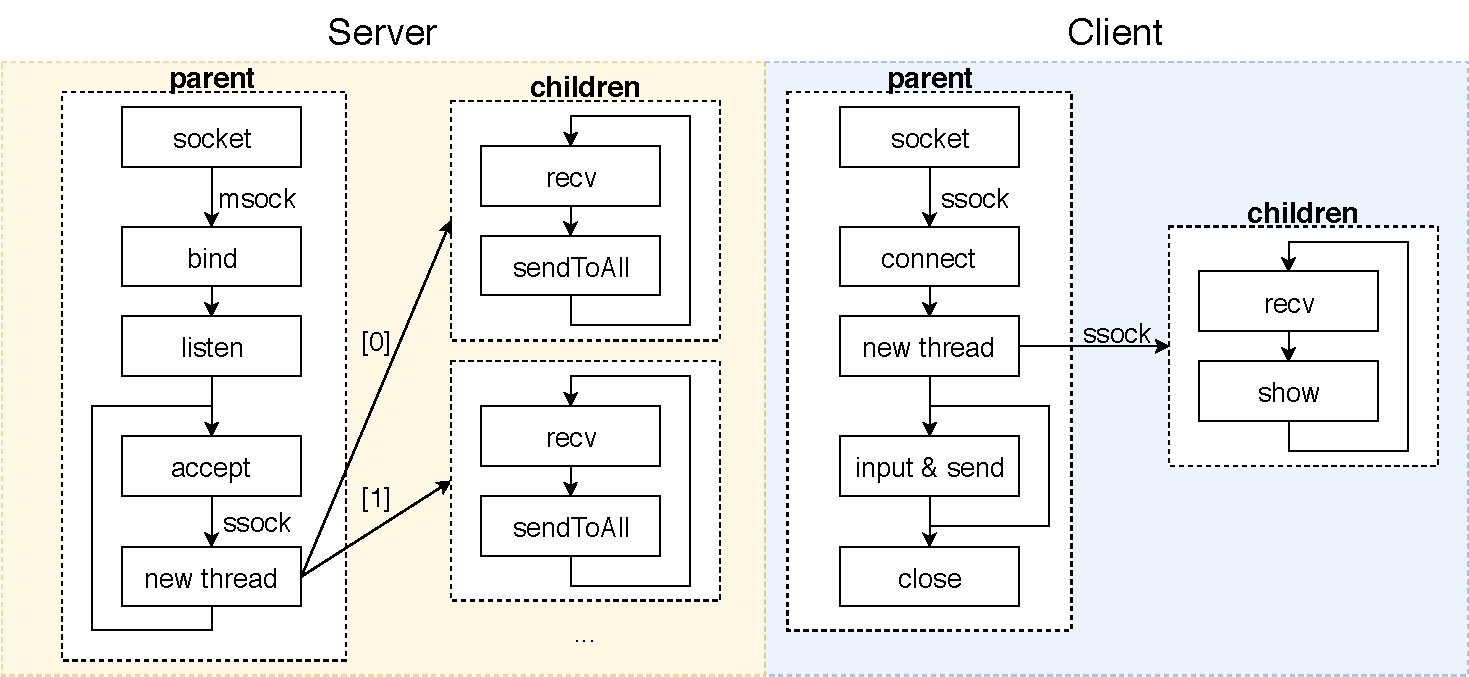
\includegraphics[width=\linewidth]{fig/socket-multithread.pdf}
\end{figure}

\subsection{多人聊天程序}
编写多人聊天程序,要求客户端和服务器都采用多线程方式进行编程。
每个客户端都采用\textbf{TCP协议}连接服务器并保持连接。
服务器同时与所有客户端建立和保持连接。
每个客户端输入的消息都会通过服务器转发给所有客户。

Linux环境下线程调用需要引入头文件\verb'<pthread.h>',同时添加编译指令\verb'-pthread'。
创建线程为\verb'pthread_create',退出线程为\verb'pthread_exit',线程等待为\verb'pthread_join'。

服务器端程序:
\begin{lstlisting}
\end{lstlisting}

客户端程序:
\begin{lstlisting}
\end{lstlisting}

在本实验中我还编写了Makefile文件,方便自动编译。
\begin{lstlisting}[language=make]
CC = gcc
FLAGS = -pthread
ALL = server client

all: $(ALL)

% : %.c
    $(CC) $(FLAGS) $< -o $@

.PHONY : clean

clean :
    -rm -f *.o $(ALL)
\end{lstlisting}

运行截屏:
% \begin{figure}[H]
% \centering
% \includegraphics[width=0.8\linewidth]
% \end{figure}

\subsection{添加信息后转发}
服务器程序转发某个客户端发来的消息时都在消息前面加上该客户端的IP地址和端口号以及服务器的当前时间。
要求服务器程序把转发的消息也显示出来。

服务器程序(修改部分):
\begin{lstlisting}
\end{lstlisting}

运行截屏:
% \begin{figure}[H]
% \centering
% \includegraphics[width=0.8\linewidth]
% \end{figure}

\subsection{``进入''信息发送}
新客户刚连接时服务器端把\verb'enter'消息(包含客户端IP地址和端口号)发送给所有客户端。

服务器程序(修改部分):
\begin{lstlisting}
\end{lstlisting}

运行截屏:
% \begin{figure}[H]
% \centering
% \includegraphics[width=0.8\linewidth]
% \end{figure}

\subsection{``退出''信息发送}
客户端输入\verb'exit'时退出客户端程序(正常退出),或者客户端直接关闭窗口退出(异常退出),服务器都会把该客户\verb'leave'的消息广播给所有客户。

服务器程序(修改部分):
\begin{lstlisting}
\end{lstlisting}

运行截屏:
% \begin{figure}[H]
% \centering
% \includegraphics[width=0.8\linewidth]
% \end{figure}

\subsection{与老师服务器连接}
运行客户端程序测试与老师的服务器程序的连接(\verb'172.18.187.9:50500')。

运行截屏(客户端):
% \begin{figure}[H]
% \centering
% \includegraphics[width=0.8\linewidth]
% \end{figure}

\subsection{与同学互测}
与同学的程序进行相互测试,一个人可以与多人测试,截屏选择其中一个。

同学的学号姓名(可以多人):17341059黄杨峻、17341111刘学海

作为服务器运行截屏:
% \begin{figure}[H]
% \centering
% \includegraphics[width=0.8\linewidth]
% \end{figure}
      
作为客户端运行截屏:
% \begin{figure}[H]
% \centering
% \includegraphics[width=0.8\linewidth]
% \end{figure}


\section{完成情况}
是否完成以下步骤?(\cmark 完成\quad\xmark 未做)
\par 1. [\cmark]\qquad 2. [\cmark]\qquad 3.[\cmark]
\par 4. [\cmark]\qquad 5. [\cmark]\qquad 6.[\cmark]

\section{实验体会}
% 写出实验过程中遇到的问题,解决方法和自己的思考;并简述实验体会(如果有的话)。


\end{document}
% 【交实验报告】
% 每位同学单独完成本实验内容并填写实验报告。
%     交作业地点:http://172.18.187.9/netdisk/default.aspx?vm=17net 
% 编程实验 
% 截止日期:2019年3月23日23:00(周六)。
% 上传文件:学号_姓名_chat实验报告.doc
% 学号_姓名_chat实验要求.rar (源程序和可执行程序)